\documentclass[a4paper, dvipdfmx]{jsarticle}
\usepackage{macros}

\usepackage{graphics}
\usepackage{tikz}
\usetikzlibrary{cd, positioning, arrows}

\newcommand{\Fib}[1]{\cat{Fib}(\cat{#1})}
\newcommand{\cFib}[1]{\cat{cFib}(\cat{#1})}
\newcommand{\sFib}[1]{\cat{sFib}(\cat{#1})}
\newcommand{\FibBP}[1]{\cat{Fib}^{\mathrm{bp}}(\cat{#1})}

\newcommand{\kiso}[1][{}]{\overset{#1}{\iso}}
\newcommand{\kequiv}[1][{}]{\overset{#1}{\simeq}}
\newcommand{\HOM}{\operatorname{HOM}}
\newcommand{\centerpb}{\ar@{}[lu]|{\text{p.b.}}}

\begin{document}
\title{ゼミノート \#4.5 \\ Fibered Categories, continued}
\author{七条彰紀}
\maketitle

\section{Cleavage}
    Cartesian liftingは普遍性(Triangle Lifting)で特徴づけられている.
    なので同型を除いて一意であるが,厳密な意味で一意であるというものではない.
    どのCartesian liftingを用いるか選んだものがCleavage(分裂,劈開).
    これはFibered category :: $\cat{X}$のCartesian arrowのclassを成す.
    Cleavageとfibration (resp. Fibered category)を併せたものを
    Cloven fibration (resp. Cloven fibered category)と呼ぶ.
    選択公理によって,我々は常にFibrationをCloven fibrationにできる.

\subsection{ Split Fibration }
    CleavageはCartesian arrowのclassであると書いたが,
    このclassが圏を成すと綺麗である.
    そのようなCleavageを選べるFibrationをSplit fibrationと呼ぶ.

    \begin{Def}[\cite{ASS}]
        $\pi \colon \cat{X} \to \cat{B}$ :: fibered categoryとする.
        splitting of $\pi$とは,以下を満たすsubcategory :: $\cat{S} \subset \cat{X}$のことである.
        \begin{enumerate}
            \item
                $\cat{S}$は$\cat{X}$の任意の対象を持つ.
            \item
                $\cat{S}$の任意の射はcartesian.
            \item
                任意の$\cat{B}$の射$f \colon U \to V$と$V$上の対象$v \in \cat{X}$について,
                $f$上の射$u \to v$がただ一つ存在する.
                (すなわち,cartesian liftingが一意に存在する.)
        \end{enumerate}
        この時,組$(\cat{X}, \cat{S})$をsplit fibered categoryと呼ぶ.
    \end{Def}

    任意のFibrationはSplit fibrationとは限らないが,Split fibrationと圏同値である.

    \begin{Thm}
        $\pi \colon \cat{X} \to \cat{B}$ :: fibered categoryとする.
        この時,split fibered category over $\cat{B}$ :: $(\tilde{\cat{X}}, \cat{S})$が存在し,
        圏同値$\tilde{\cat{X}} \kequiv \cat{X}$が成立する.
    \end{Thm}

    \begin{proof}
        ここでは
        圏と部分圏$(\tilde{\cat{X}}, \cat{S})$及び
        関手$\Phi \colon \tilde{\cat{X}} \to \cat{X}$を構成するにとどめる.
        (TODO: 
        これらがそれぞれsplit fibered category over $\cat{B}$とequivalenceであることは
        ここでは確認しない.)

        以下のように$\tilde{\cat{X}}$を構成する.
        \begin{description}[labelindent=1cm]
            \item[Objects.]
                object :: $U \in \cat{B}$と
                morphism of fibered category :: $u \colon \cat{B}/U \to \cat{X}$の組$(U, u)$.

            \item[Arrows.]
                射$(V, v) \to (U, u)$は
                $\cat{B}$の射$g \colon V \to U$と
                base-preserving isomorphism :: $\alpha \colon v \to u \circ g$の組$(g, \alpha)$.
                \begin{center}
                \begin{tikzcd}
                    \cat{B}/V \ar[r, "g"] \ar[rr, bend right=40mm, "v"'{name=v}]
                    & \cat{B}/U \ar[Rightarrow, from=v, "\alpha"]\ar[r, "u"]
                    & \cat{X}
                \end{tikzcd}
                \end{center}
        \end{description}

        まずprojection functorが以下のように定まる.
        \begin{defmap}
            \tilde{\pi} \colon & \tilde{\cat{X}}& \to& \cat{B} \\
            {}& (U, u)& \mapsto& U
        \end{defmap}
        この関手によってfibered categoryの構造が入る.

        さらに次の関手によってequivalenceが与えられる.
        \begin{defmap}
            \Phi\colon & \tilde{\cat{X}}& \to& \cat{X} \\
            {}& (U, u)& \mapsto& u(\id[U])
        \end{defmap}
        これがequivalenceであることは$2$-Yoneda Lemmaによる.

        最後に,splitting of $\tilde{\pi}$ :: $\cat{S}$が次で定められる.
        \begin{description}[labelindent=1cm]
            \item[Objects.]
                $\tilde{\cat{X}}$と同じ.

            \item[Arrows.]
                $\tilde{\cat{X}}$の射で,$(g, \id)$と表されるもの.
                すなわち,
                射$(V, v) \to (U, u)$は$\cat{B}$の射$g \colon V \to U$であって
                $v=u \circ g$であるもの.
                \begin{center}
                \begin{tikzcd}
                    \cat{B}/V \ar[r, "g"] \ar[rr, bend right=40mm, "v"'{name=v}]
                    & \cat{B}/U \ar[equal, from=v]\ar[r, "u"]
                    & \cat{X}
                \end{tikzcd}
                \end{center}
        \end{description}
    \end{proof}

    \begin{Def}
        圏$\cat{B}$に対し,
        \begin{itemize}
            \item Cloven fibration over $\cat{B}$の圏を$\cFib{B}$,
            \item Split fibration over $\cat{B}$の圏を$\sFib{B}$
        \end{itemize}
        と書く.
        ぞれぞれ忘却関手$\sFib{B} \to \cFib{B}, \cFib{B} \to \Fib{B}$をもつ.
    \end{Def}

\section{Grothendieck Construction} \label{sec:gro_const}
    今,fibered categoryからfiberとしてpsuedo-functorを構成した.
    実はこの逆が出来る.
    \begin{Def}[Grothendieck Construction, \cite{ASS}, \cite{IntroFibCat}]
        psuedo-functor :: $P \colon \cat{B} \to \Cat/\cat{B}$について,
        以下のように圏$\int P$を定義する.
        \begin{description}[labelindent=1cm]
            \item[Object.] $b \in \cat{B}$と$x \in P(b)$の組$(b, x)$.
            \item[Arrow.] $\phi \colon b \to b'$と$\Phi \colon P(\phi)(x) \to x'$の組$(\phi, \Phi)$.
        \end{description}
        射の合成は$(\psi, \Psi) \circ (\phi, \Phi)=(\psi \circ \phi, \Phi \circ P(\psi)(\Phi))$で与えられる.
        
        この圏によって以下の関手が定まる.
        \begin{defmap}
            \int \colon & \left\{ \parbox{2.3cm}{psuedo-functor \\ \quad \ $\cat{B} \to \Cat$} \right\}&
                \to& \sFib{B} \\
            {}& P& \mapsto& \int P
        \end{defmap}
    \end{Def}

    \begin{Example}
        scheme :: $S$について,
        representable functor :: $\ftor{S}$は$\Sch/S$に対応する.
    \end{Example}

    \begin{Example}
        presheaf of set :: $F \colon \cat{C} \to \Sets$は
        $\bigsqcup_{c \in \cat{C}} F(c)$に対応する.
    \end{Example}

    \begin{Remark}
        David I. Spivak ``Category theory for scientists"によると,
        Grothendieck Constructionを最初に構成したのはGrothendieckではない.
        例えばMacLaneが以前から扱っている.
    \end{Remark}

    \begin{Def}[weak/strict $2$-equivalence]
        関手$F \colon \cat{C} \rightarrow \cat{D}$が
        weak $2$-equivalenceであるとは,以下が成り立つこと:
        逆向きの関手$\cat{C} \leftarrow \cat{D} \colon G$と
        二つの自然変換$\alpha \colon GF \to \id[\cat{C}], \beta \colon FG \to \id[\cat{D}]$が存在し,
        \begin{itemize}
            \item 各$c \in \cat{C}, d \in \cat{D}$について$\alpha_{c}, \beta_{d}$は同型であり,
            \item 射$\phi \in \Arr(\cat{C}), \psi \in \Arr(\cat{D})$について$\alpha_{\phi}, \beta_{\psi}$も同型.
        \end{itemize}
        $\alpha_{\phi}, \beta_{\psi}$が恒等射であるときはstrict $2$-equivalenceという.
    \end{Def}

    \begin{Thm}[Grothendieck Construction give Category Equivalence]
        Grothendieck Construction
        \[
            \int \colon
            \left\{ \parbox{2.3cm}{psuedo-functor \\ \quad \ $\cat{B} \to \Cat$} \right\} \to \cFib{B}
        \]
        はstrict $2$-equivalenceである.
        また,このあとに忘却関手$\cFib{B} \to \Fib{B}$を続けると,
        weak $2$-equivalenceとなる.
    \end{Thm}
    \begin{proof}
        \cite{NoteGroTop} \S 3.1.3に詳しい証明がある.
        あるいは,
        P. T. Johnstone
            ``Sketches of an Elephant: A Topos Theory Compendium vol.1 (Oxford Logic Guides 43)"
        に証明がある.
    \end{proof}
    
    \begin{Remark}
        $\Fib{B}$と``anafunctor"の圏がstrict $2$-equivalenceである,
        という述べ方もあるようだが,
        ``anafunctor"を用いる理由が特に無いので,このノートでは導入しない.
    \end{Remark}

    \begin{Remark}
        この定理から,
        psuedo-functorの理論とfibered categoryの理論は殆ど同じ,と言える.
        また,今後現れるstackなどはpsuedo-functorに対して定義され,
        一見,fibered categoryの理論は扱う必要性がなくなる.
        
        しかし実際には,fibered categoryの方がpsuedo-functorより構成しやすい,
        あるいは全体の性質を理解しやすいという面がある.
        また技術的な有利としては,
        fibered categoryはcleavage(例えばpullback, fiber product等)を選択する必要がなく,
        例えば,pullbackの貼り合わせ(貼り合わせの際には同型での変形が必要に成る)を自然に扱うことが出来る
        \footnote
        {
            もう少し具体的な例としては,
            trivial familyの貼り合わせで出来るlocally trivial familyも扱える.
            詳しい例は私のDeformation Theoryに関するノートを読んで欲しい.
        }.
        
        また,直観としては,fibered categoryはfamilyである.
        ここから得られるfiberは正にfiber of familyである.
        そのためfibered categoryは大域的,psuedo-functorは局所的だと考えられる.

        (TODO: あとで分かったらもっと追記する.)
    \end{Remark}

\section{Category Fibered in Groupoids/Sets}
\subsection{Motivation}
    Category Fibered in Groupoidsは「綺麗すぎる」fibered categoryであるが,
    我々が研究する範囲では珍しいものではない.
    

\subsection{Definition}
    \begin{Def}[Groupoid]
        任意の射が同型射である圏をgroupoidと呼ぶ.
    \end{Def}

    \begin{Remark}
        群は対象がただ一つで任意の射が同型であるものとみなせるため,
        groupoidにはこの名前がある.

        群以外の極めて単純なgroupoidとして,
        集合を射が恒等射しかない圏(離散圏)とみなしたものがある.
        そのため,逆に恒等射しか無い圏もsetと呼ぶ.
    \end{Remark}

    \begin{Def}[Category fibered in groupoids/sets]
        $\pi \colon \cat{X} \to \cat{B}$をfibered categoryとする.
        任意の$b \in \cat{B}$について,
        $\pi$の$b$におけるfiber$\cat{X}(b)$がgroupoid (set)であるとき,
        $\cat{X}$をcategory fibered in groupoids (sets)と呼ぶ.
    \end{Def}
    category fibered in groupoidsは次のように定義しても同値である.

    \begin{Def}[Category fibered in groupoid (Another Definition)]
        任意の射がcartesianであるfibered categoryをcategory fibered in groupoidsと呼ぶ.
        すなわち,
        以下の$2$条件が成立する圏$\cat{X}$と関手$\pi \colon \cat{X} \to \cat{B}$を
        category fibered in groupoidsと呼ぶ.
        \begin{enumerate}[label=(\roman*)]
        \item
            以下の図式(1)において,
            上の箱と下の箱が$\pi$で対応し,下の箱にある図式が可換であるとする.
            この時,図式(2)のように上の箱にある図式を可換にし,
            $\pi$での対応を保つ射$z \to x$がただ一つ存在する.
            %% {{{
            \begin{center}
            \begin{tikzpicture}[mybox/.style={draw, inner sep=5pt}]
            \node[mybox] (X) at (0,3){%
                \begin{tikzcd}
                    {} & z \ar[rd]& {} \\
                    x \ar[rr] &{}& y
                \end{tikzcd}
            };
            \node[mybox] (B) at (0,0){%
                \begin{tikzcd}
                    {} & \pi(z) \ar[rd]\ar[ld]& {} \\
                    \pi(x) \ar[rr] &{}& \pi(y)
                \end{tikzcd}
            };

            \node [above=5pt of X] {in $\cat{X}$};
            \node [below=5pt of B] {in $\cat{B}$};
            \draw [->, line width=1.5pt] (X) edge (B);
            \node at (0.3,1.55) {$\pi$};
            \draw (4,4) -- (4,-1);
            \node at (-3,4) {($1$)};
            \end{tikzpicture}
            \qquad \qquad
            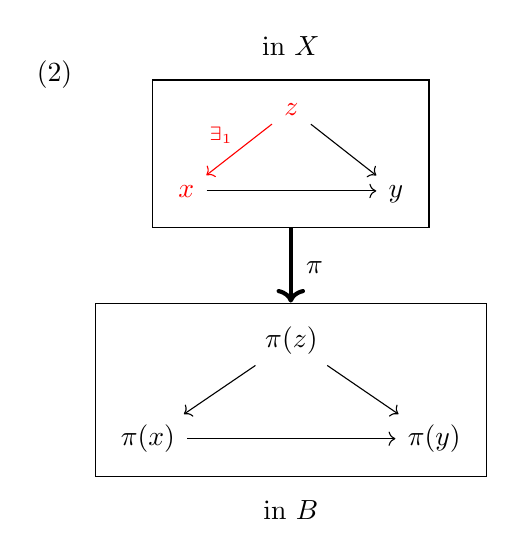
\begin{tikzpicture}[mybox/.style={draw, inner sep=5pt}]
            \node[mybox] (X) at (0,3){%
                \begin{tikzcd}
                    {} & \color{red}z \ar[rd] \ar[ld, red, "\exists_1"']& {} \\
                    \color{red}x \ar[rr] &{}& y
                \end{tikzcd}
            };
            \node[mybox] (B) at (0,0){%
                \begin{tikzcd}
                    {} & \pi(z) \ar[rd]\ar[ld]& {} \\
                    \pi(x) \ar[rr] &{}& \pi(y)
                \end{tikzcd}
            };

            \node [above=5pt of X] {in $\cat{X}$};
            \node [below=5pt of B] {in $\cat{B}$};
            \draw [->, line width=1.5pt] (X) edge (B);
            \node at (0.3,1.55) {$\pi$};
            \node at (-3,4) {($2$)};
            \end{tikzpicture}
            \end{center}
            %% }}}

        \item
            $y \in \cat{X}, u \to \pi(y) \in \cat{B}$に対し,
            以下の図式を満たす
            \footnote{すなわち,$\pi(x)=u, \pi(x \to y)=u \to \pi(y)$を満たす.}
            \underline{$x \in \cat{X}$と射$x \to y \in \cat{X}$}が存在する.
            \begin{center}
            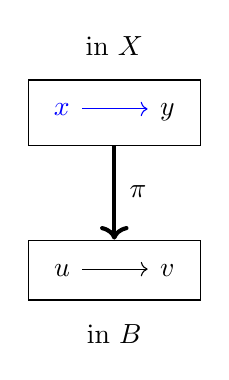
\begin{tikzpicture}[mybox/.style={draw, inner sep=5pt}]
            \node[mybox] (X) at (0,2){%
            \begin{tikzcd}
                \color{blue}x \ar[r, blue]& y
            \end{tikzcd}
            };
            \node[mybox] (B) at (0,0){%
            \begin{tikzcd}
                u \ar[r]& v
            \end{tikzcd}
            };

            \node [above=5pt of X] {in $\cat{X}$};
            \node [below=5pt of B] {in $\cat{B}$};
            \draw [->, line width=1.5pt] (X) edge (B);
            \node at (0.3,1) {$\pi$};
            \end{tikzpicture}
            \end{center}
        \end{enumerate}
    \end{Def}


\section{Fiber Product of Category Fibered in Groupoids}
    (ここで扱おうと思ったが,今は扱うモチベーションがないので後回しにする.)
%    \begin{Thm}
%        Category fibered in groupoidsの圏はfiber productを持つ.
%    \end{Thm}
%    \begin{Remark}
%        特別なCategory fibered in groupoidsがstack(次のセミナーで定義する)であるから,
%        この定理は,schemeのfiber productの存在の一般化である.
%    \end{Remark}
%    \begin{proof}
%        具体的に新しい構成し,
%    \end{proof}

\section{Equivalence of Fibered Categories}
    Fibered categoryの一般論の最後に,
    この直後に扱うことと成るEquivalenceを扱う.
    
    この節では
    fibered categories :: $\pi \colon \cat{X} \to \cat{B}, \pi' \colon \cat{X}' \to \cat{B}$と,
    これらの間の射$g \colon \cat{X} \to \cat{X}'$を考える.

\subsection{Definition}
    \begin{Def}[Equivalence]
        $g$がequivalence of fibered categoriesであるとは,
        別の射$h \colon \cat{X}' \to \cat{X}$が存在し,
        $g \circ h, h \circ g$が
        それぞれ恒等関手とbase-preserving isomorphicであるということである.

        この時,$\cat{X} \simeq \cat{X}'$と書き,
        $h$はpsuedo-inverse of $g$と呼ばれる.
    \end{Def}
    \begin{Remark}
        比較すれば分かるとおり,
        equivalence of fibered categoriesは,
        通常の圏同値の定義に``base-preserving"という条件が追加されただけである.
    \end{Remark}

\subsection{Propositions}
    \begin{Prop}
        fiberedとは限らない圏$\cat{C}, \cat{D}$と
        その間の関手$F \colon \cat{C} \to \cat{D}$について,
        $F$が圏同値であることは以下の$2$条件が同時に成立することと同値.
        \begin{description}
            \item[Fully Faithfulness.] \mbox{}\\
                任意の$c,c' \in \cat{C}$について,\mbox{}\\
                関手$F$が与えるclassの対応$\Hom_{\cat{C}}(c, c') \to \Hom_{\cat{D}}(F(c), F(c'))$は全単射である.

            \item[Essential Surjectivity.] \mbox{}\\
                任意の$d \in \cat{D}$について,$F(c) \iso d$となる対象$c \in \cat{C}$が存在する.
        \end{description}
    \end{Prop}
    \begin{proof}
        \cite{Awodey} Prop7.26を参照せよ.
    \end{proof}

    \begin{Prop}[\cite{ASS} Prop3.1.18, 3.1.10]
        $b \in \cat{B}$について,
        $g$を$\cat{X}(b)$に制限して得られる関手を$g_b \colon \cat{X}(b) \to \cat{X}'(b)$とする.
        \begin{enumerate}[label=(\alph*)]
        \item $g$ :: fully faithful
                $\iff$ 任意の$b \in \cat{B}$について,$g_{b}$ :: fully faithful.
        \item $g$ :: equivalence
                $\iff$ 任意の$b \in \cat{B}$について,$g_{b}$ :: equivalence
                    \footnote{こちらは通常の圏同値}.
    \end{enumerate}
    \end{Prop}
    \begin{proof}
        いずれも$\implies$は自明なので$\impliedby$を示す.

        (i)の証明の概略は以下の通り.
        まず$\Hom_{\cat{C}}(c, c'), \Hom_{\cat{D}}(F(c), F(c'))$を
        \begin{align*}
            \Hom_{\cat{C}}(c, c')
            =&\bigsqcup_{h \in \Hom_{\cat{B}}(\pi(c), \pi(c'))}
            \left\{\parbox{2.85cm}{morphisms $c \to c'$, \\ \qquad\ \ over $h$}\right\}, \\
            \Hom_{\cat{D}}(F(c), F(c'))
            =&\bigsqcup_{h \in \Hom_{\cat{B}}(\pi(c), \pi(c'))}
            \left\{\parbox{4cm}{morphisms $F(c) \to F(c')$, \\ \qquad\qquad\ over $h$}\right\}
        \end{align*}
        と分解する.
        そして各$h$についてsession 4の命題4.2
        (射はcartesian arrowと$\id$に写る射の合成に分解できる)を用いる.
        すると各成分について全単射を構成できる.

        (TODO: proof of (ii))
    \end{proof}

\bibliographystyle{jplain}
\bibliography{reference}
\end{document}
